\documentclass[tikz]{standalone}
\usepackage{pgfplots}
%\pgfplotsset{compat=1.8}
\begin{document}

\pgfplotsset{
    every axis/.append style={font=\tiny},
}

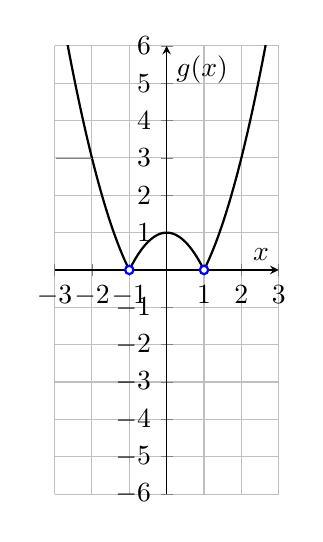
\begin{tikzpicture}[
  declare function={
    % define the arctan function, be sure to include rad() so as radians are used
    linear(\x)= x^2-1;
    flipped(\x)= abs(x^2-1);
  }
]
\begin{axis}[
  axis equal image,
  grid=major,
  axis x line=middle,
  axis y line=middle,
  xmin=-3, xmax=3, xtick={-3,...,3},
  xlabel=$x$,
  ymin=-6, ymax=6, ytick={-6,...,6},
  ylabel=$g(x)$,
]

%\pgfplotsinvokeforeach{-1.570796, -0.785398, 0.785398, 1.570796 }{
%  \draw[dotted] ({axis cs: -5, #1}) -- ({axis cs: 5, #1});}

\addplot[black, domain=-3:-1, smooth, thick]{linear(x)};
\addplot[black, domain=1:3, smooth, thick]{linear(x)};
\addplot[black, domain=-1:1, smooth, thick]{flipped(x)};

\draw [draw=blue, fill=white, thick] (axis cs: -1, 0) circle (1.5pt);
\draw [draw=blue, fill=white, thick] (axis cs: 1, 0) circle (1.5pt);

\node[coordinate,pin=left:{Good!}]
    at (axis cs:-2,3) {};

\end{axis}

\end{tikzpicture}

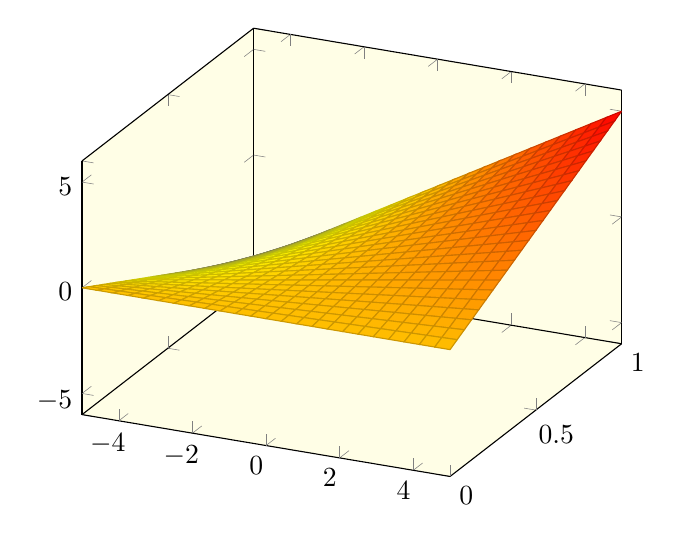
\begin{tikzpicture}
    \begin{axis}[
        axis background/.style={fill=yellow!10}]
    \addplot3[surf,y domain=0:1]
        {x*y};
    \end{axis}
\end{tikzpicture}

\end{document}